\section{The two-depth potential}\label{ledger:section}

The reductions of Proposition~\ref{rec:reductions} have three transitions
with potentially positive cost.  For a suffix step \([a,t]\to[a,p]\),
if a depth to the left of the policy's inner interval minimizes \(A\)
on both intervals, the minimum does not increase and cannot pay a
positive cost \(A_p-\min_{[p,t]}A\).  We instead use a pair of well-separated
depths.  In a suffix child, separation places the later depth in the
inner interval, so it can be replaced by a minimizer on \([p,t]\)
while the earlier depth remains.  A high prefix or direct reduction can
replace the earlier depth.

\begin{definition}[Two-depth potential]\label{ledger:potential}
For an integer interval \(J=[a,t]\) of width at least \(10q_0\), put
\begin{equation}\label{ledger:potential-formula}
 \mathcal V(J)=
 \min_{\substack{a\le i<j\le t\\j-i\ge10q_0}}(A_i+A_j).
\end{equation}
We leave \(\mathcal V(J)\) undefined for shorter intervals.
\end{definition}

The potential is attached to the current interval: \([a,t]\) for
\(\mathsf D_i(a,t)\) and \([a,v]\) for
\(\mathsf H_i^{\mathcal B}(a,v)\).
The retained base \(\mathcal B\) supplies the angular state's descriptor
list, from which the reached anchors have been removed; the origin of a chosen descriptor
supplies the inner interval on which its anchor minimizes \(A\).
Neither replaces the current interval in the payment inequality.

\begin{lemma}[Payment of the costs]\label{ledger:payment}
If a reduction of Proposition~\ref{rec:reductions} has a potentially
positive cost and parent interval \(J\) and child interval \(J'\),
then \(\mathcal V(J')\) is defined and
\begin{equation}\label{ledger:payment-inequality}
 \mathrm{cost}\le\mathcal V(J')-\mathcal V(J).
\end{equation}
For every zero-cost reduction whose child potential is defined,
the same inequality holds.
\end{lemma}

\begin{proof}
Containment of the admissible pairs immediately gives
\(\mathcal V(J)\le\mathcal V(J')\) when \(J'\subset J\) and
both potentials are defined.  This proves all zero-cost cases.
We check the other cases by replacing one depth in an arbitrary
admissible child pair, then apply the result to a minimizing child
pair.  Only the inner-interval minimizing property of the policy is
needed; no monotonicity of \(A\) is assumed.

\paragraph{Suffix.}
Here \(J=[a,t]\), \(J'=[a,p]\), and
\(\mathrm{cost}=A_p-\min_{[p,t]}A\).
Since \(2p>a+t\), the child width is more than half the nonterminal
parent width, and hence greater than \(10q_0\).
Let \((i,j)\) be admissible in \([a,p]\).  Then
\(j\ge a+10q_0\), while the left endpoint of the origin's inner
interval is at most \(a+2q_0\).  Since \(j\le p\), the index
\(j\) belongs to that inner interval, so \(A_j\ge A_p\).
Choose \(r\in[p,t]\) attaining \(\min_{[p,t]}A\).
The pair \((i,r)\) is admissible in the parent because
\(r\ge j\), and
\[
 A_i+A_r\le A_i+A_j-
          \left(A_p-\min_{[p,t]}A\right).
\]
This gives \eqref{ledger:payment-inequality}.

\paragraph{High prefix.}
Here \(J=[a,t]\), \(J'=[p,v]\), \(t-v<\sigma N\), and the
cost is \(k(a,p)\).  The prefix inequality gives
\[
 v-p\ge(t-a)/2-\sigma N>10q_0.
\]
For an admissible child pair \((i,j)\),
\(p\le i\le v-10q_0\le t-10q_0\).  Thus \(i\) is in the
origin's inner interval and \(A_i\ge A_p\).
Choose \(r\in[a,p]\) attaining \(\min_{[a,p]}A\).
The pair \((r,j)\) stays in \([a,t]\) and remains admissible,
because \(r\le i\).  Its sum is at most
\(A_i+A_j-k(a,p)\), as required.

\paragraph{Direct graph reduction.}
Now \(J=[a,v]\), \(J'=[p,v]\).  Let \(L\) be the maximal
remaining descriptor length chosen by the reduction, and let
\([b_0,u_0]\) be its origin.  We have
\begin{equation}\label{ledger:origin-geometry}
 b_0\le p-L,\qquad p+L\le u_0,
 \qquad v\le a+2L.
\end{equation}
The reduction gives \(v-p\ge(v-a)/2-\sigma N\).
Nonterminality and \(\sigma\ll\kappa\) make this greater than \(10q_0\).
If \(k(a,p)=0\), containment suffices.  Otherwise choose
\(i_0\in[a,p]\) with
\[
 A_{i_0}=\min_{[a,p]}A=A_p-k(a,p)<A_p.
\]
The origin's policy makes \(A_p\) no larger than every value in
its inner interval.  Since \(i_0\le p\), the index \(i_0\)
must lie strictly to the left of that inner interval, whether or
not it lies in the origin itself.  Consequently
\[
 a\le i_0<b_0+2q_0,
 \qquad
 v\le a+2L<b_0+2q_0+2L\le u_0+2q_0.
\]
For any admissible child pair \((i,j)\),
\[
 p\le i\le v-10q_0<u_0-8q_0.
\]
The origin's inner interval begins no later than \(p\) and ends
no earlier than \(u_0-2q_0\).  Therefore \(i\) lies in it, and
\(A_i\ge A_p\).  Replacing \(i\) by \(i_0\) gives a pair
\((i_0,j)\) in the \emph{actual parent} \([a,v]\), not merely in
the origin.  It remains admissible because \(i_0\le p\le i\),
and its sum decreases by at least \(k(a,p)\).  This proves the
direct case.
\end{proof}

\begin{figure}[t]
 \centering
 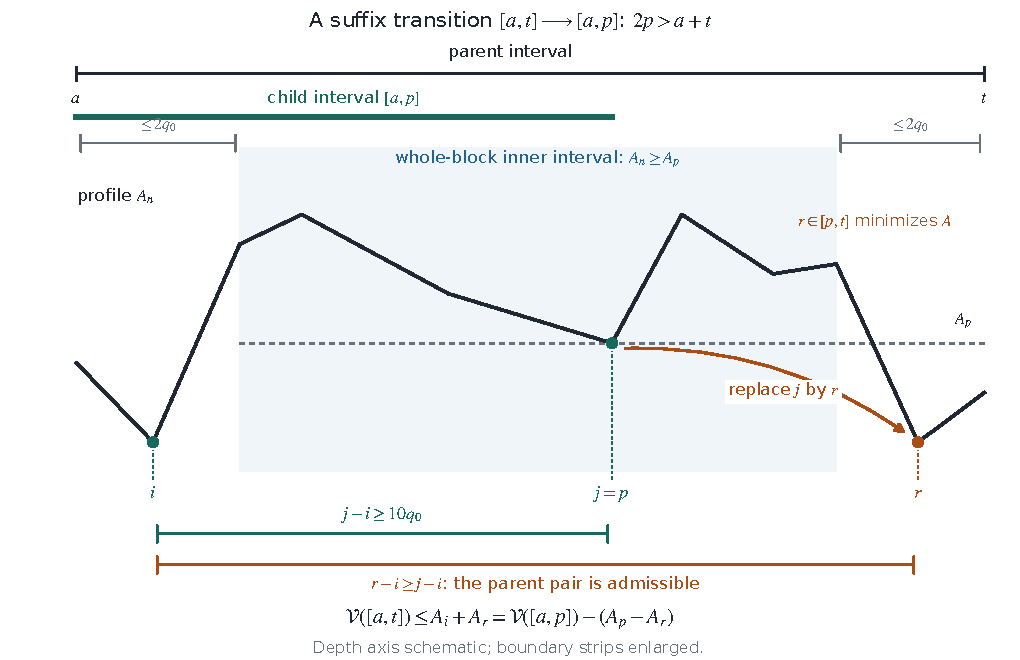
\includegraphics[width=\textwidth]{figures/potential-replacement.pdf}
 \caption{Payment for a suffix transition in Lemma~\ref{ledger:payment}.
 Replacing the later depth of a minimizing child pair by the inner-interval
 minimizer $p$ preserves separation and cannot increase the sum. Thus a
 minimizing child pair can be chosen as $(i,p)$. If $r$ minimizes $A$ on
 $[p,t]$, the pair $(i,r)$ is
 admissible in the parent. Its sum is lower by $A_p-A_r$, which pays the
 transition cost. A positive drop places $r$ beyond the inner interval.
 The depth axis is schematic, with the boundary strips enlarged.}
 \label{fig:potential-replacement}
\end{figure}


\begin{lemma}[Finite policy and smoothing budget]\label{ledger:termination}
Every branch of the state reductions has at most \(20/\kappa\)
non-low transitions and at most \(1/\sigma\) low transitions, for
sufficiently small fixed parameters and sufficiently large \(N\).
Along such a branch the smoothing index increases by at most
\(20/\kappa+1/\sigma\).  If the initial index is zero, every index
required by the iteration, including the next support level used by
a mask, is less than
\[
 J_0=\left\lceil100(1/\kappa+1/\sigma)+100\right\rceil.
\]
\end{lemma}

\begin{proof}
Along a branch the start depth never decreases and the end depth
never increases.  Let \(K\) be the number of fixed block
representatives; for large \(N\), \(K\le1/\kappa+2\).
Every high or direct step strictly advances the start to a
representative.  Such a representative can never be passed twice,
so together these steps number at most \(K\).  Each suffix step
lowers the end by at least \(q_0\), and therefore there are at most
\(N/q_0\le1/\kappa\) suffix steps.  Low steps lower the end by
at least \(\sigma N\), so there are at most \(1/\sigma\).

An angular episode starts at the root or immediately after a high
step and ends at a far step or a stopping term.  Direct and near
steps remain in that episode.  There are at most \(K+1\) episodes,
and hence at most \(K+1\) far steps.

Consider a near step whose child is nonterminal.  That child has
width \(2L_0>100q_0\), so the floor in the formula for \(L_0\)
is inactive and \(L=L_0\).  Remove the factors whose anchors have
now been reached.  If the maximum remaining nominal length
decreases, at least one formerly maximal anchor has just been
passed; charge the near step to one such anchor.  These charges
are distinct along the branch.  If the maximum stays equal to
\(L\), recomputing \(v-2L\) at the child gives exactly its start
depth, so the very next step is direct.  Charge this near step to
that next direct step.  Finally there is at most one near step
with terminal child.  Thus near steps number at most \(2K+1\).
The combined non-low count is at most \(5K+2\), which is less
than \(20/\kappa\) for sufficiently small \(\kappa\).

Only suffix, low, and far steps increase the smoothing index;
each increases it by one.  If \(i_{\mathrm{in}}\) is the initial
index, the preceding counts therefore give
\[
 i\le i_{\mathrm{in}}+20/\kappa+1/\sigma
\]
at every state on the branch.  High, direct, and near steps use the
level-\(i+1\) supports of their index-\(i\) symbols without increasing
the index.  For \(i_{\mathrm{in}}=0\), even this additional support
level remains below \(J_0\), since
\(20/\kappa+1/\sigma+1<J_0\).  Thus every mask and support level
required for the iteration from index zero is available.
\end{proof}

\begin{theorem}[Single-profile angular bound]\label{ledger:bound}
Let \(\mathsf H_0^{[c,N]}(c,N)\) be a recursive angular state of
nonterminal width, as in Definition~\ref{rec:angular-state}.
Fix its initial derivative budget \(B\) and its common numerical angular
bounds \(Q_j\), independently of \(N\), as in
Definition~\ref{osc:symbols}.
Then
\begin{equation}\label{ledger:bound-equation}
 \mathsf H_0^{[c,N]}(c,N)
 \le R^{2A_c-\mathcal V([c,N])
                   +C_d(\kappa+\sigma/\kappa)+o(1)}.
\end{equation}
This bound holds uniformly over its two occupied cells, including
two copies of the same cell, and over its admissible bounded
spatial multipliers and symbols with these fixed bounds.  The \(o(1)\)
term may depend on \(B\) and the \(Q_j\).
\end{theorem}

\begin{proof}
Iterate Proposition~\ref{rec:reductions}, stopping at every terminal
state or low-frequency stopping term.  Lemma~\ref{ledger:termination}
gives a depth bound depending only on the fixed parameters.  Since the
root index is zero, it also ensures that every index required to continue
a nonterminal child is available.
Each transition has at most polynomially many discrete choices
in \(N\), and all coefficient sums in the oscillatory estimates
are bounded or subpower.  Thus the total main term is bounded by
\(R^{o(1)}\) times the largest terminal branch bound.  Suprema
over symbol classes are already part of the transition bounds
and require no count of the members of those classes.

Fix a branch, and let \(a_f\) be its final start.  The changes
of start in \eqref{rec:transition-factor} telescope exactly to
\(2A_c-2A_{a_f}\).  By Lemma~\ref{ledger:payment}, all costs
are bounded by increases in the potential while it is defined.
If a child has width less than \(10q_0\), it is already terminal;
moreover, the step reaching it has zero cost, since every
potentially positive-cost child has width greater than
\(10q_0\).  Let \(J_*=[u,w]\) be the last interval on the
branch with defined potential.  Then
\begin{equation}\label{ledger:cost-sum}
 \sum\mathrm{cost}
 \le\mathcal V(J_*)-\mathcal V([c,N]).
\end{equation}
This also applies when a low-frequency term stops at a
nonterminal interval.

We estimate \(\mathcal V(J_*)\) directly; no potential is assigned
to a shorter final interval.  Nesting gives \(a_f\in[u,w]\), and
\(w-u\ge10q_0\).  Set
\[
 i=\max\{u,\min\{a_f,w-10q_0\}\},\qquad j=i+10q_0.
\]
Both indices lie in \(J_*\), they are separated by \(10q_0\),
and each is within \(10q_0\) of \(a_f\).  The profile Lipschitz
bound therefore gives
\begin{equation}\label{ledger:last-potential}
 \mathcal V(J_*)\le A_i+A_j
 \le2A_{a_f}+20d\,q_0/N
 =2A_{a_f}+O_d(\kappa)+o(1).
\end{equation}
Combining \eqref{ledger:cost-sum}--\eqref{ledger:last-potential}
with the telescoping start factors leaves
\(2A_c-\mathcal V([c,N])+O_d(\kappa)+o(1)\).
The stopping bound contributes \(O_d(\kappa+\sigma)\).
Only non-low transitions incur \(C_d\sigma\) slack, so their
combined loss is \(O_d(\sigma/\kappa)\), by
Lemma~\ref{ledger:termination}.  Low transitions contribute only
subpower factors.  This proves the main-term estimate in
\eqref{ledger:bound-equation}.

For completeness, we fix the error and derivative budgets before
taking \(N\) large.  Since \(m\) is nondecreasing and
\(d\)-Lipschitz with \(m(0)=0\), all differences of \(A\) and
all costs in the reductions are bounded in absolute value by a
dimensional constant.  Each ancestor main factor is consequently
at most \(R^{C_d+o(1)}\).  Choose a target accuracy
\[
 T>C_d(1/\kappa+1/\sigma)+10d+10,
\]
with the dimensional constant large enough for the branch bound.
Demand this accuracy after all single-step normalizations and
sums.  Lemma~\ref{ledger:termination} then ensures that every
propagated additive error is negligible relative to the right
side of \eqref{ledger:bound-equation}.

There is no recursive increase of the persistent angular
derivative budget.  Each passage from a positive distance count
to an angular state begins with fresh undifferentiated masks;
choose its inverse stationary expansion order first, large
enough for the prescribed \(T\).  The resulting finite order,
together with the initial order in the Theorem, bounds all
derivatives carried by angular states.  The common bounds for the smooth
angular factors can likewise be fixed from the initial \(Q_j\) and the
bounds in Proposition~\ref{osc:shell-conversion} at the fixed accuracy
used for these conversions.
The graph estimate returns the original symbols restricted to child cells,
with no additional derivatives.  Removing reached
factors from its positive child energy, as in a near transition, adds
no derivatives to the remaining symbols.  A far step may use
an arbitrarily long direct stationary expansion, but its child
is a positive distance count and carries none of those
derivatives.  Choose the nonstationary integration orders and
the direct stationary orders after this persistent budget has
been fixed.  They may depend on \(d,\kappa,\sigma,T\) and the
initial budget, but not on \(N\).  Their large constants and
polynomial descriptor counts are absorbed in the permitted
constant and \(o(1)\) terms; the dimensional exponent losses in
the preceding algebra are unchanged.  The asserted bound
follows.
\end{proof}
